\documentclass[10pt,twocolumn,letterpaper]{article}

\usepackage{dependable_dnn}
\usepackage{times}
\usepackage{epsfig}
\usepackage{graphicx}
\usepackage{amsmath}
\usepackage{amssymb}
\usepackage{bbm}
\usepackage{subfigure}
\usepackage[table, dvipsnames]{xcolor}

% Include other packages here, before hyperref.

% If you comment hyperref and then uncomment it, you should delete
% egpaper.aux before re-running latex.  (Or just hit 'q' on the first latex
% run, let it finish, and you should be clear).
\usepackage[pagebackref=true,breaklinks=true,letterpaper=true,colorlinks,bookmarks=false]{hyperref}

\DeclareMathOperator*{\argmin}{arg\,min}
\newcommand{\Rho}{\mathrm{P}}
\newcommand{\indic}[1]{\mathbbm{1}_{\{#1\}}}
\newcommand{\closs}[1]{{\cal L}_{\rm class}(#1)}
\newcommand{\bloss}[1]{{\cal L}_{\rm box}(#1)}

\iccvfinalcopy % *** Uncomment this line for the final submission

\def\iccvPaperID{} % *** Enter the Paper ID here
\def\httilde{\mbox{\tt\raisebox{-.5ex}{\symbol{126}}}}

% Pages are numbered in submission mode, and unnumbered in camera-ready
\ificcvfinal\pagestyle{empty}\fi

\begin{document}

%%%%%%%%% TITLE - PLEASE UPDATE
\title{AdaFuse: Adaptive Temporal Fusion Network for Efficient Action Recognition\\ {\rm {\normalsize Seungmin Lee (profile2697@gmail.com; 2020-20866), \\Dept. of Electrical and Computer Engineering, Seoul National University}}}   % **** Enter the paper title and student information here

\maketitle
\thispagestyle{empty}

\section{Introduction and Motivation}
In video action recognition, both temporal modeling and employing temporal redundancy are crucial. For the purposes, the authors propose AdaFuse, named from an adaptive temporal fusion network, that dynamically selects and fuses the channels of current and past feature maps. 

\begin{figure}[b]
	\centering
	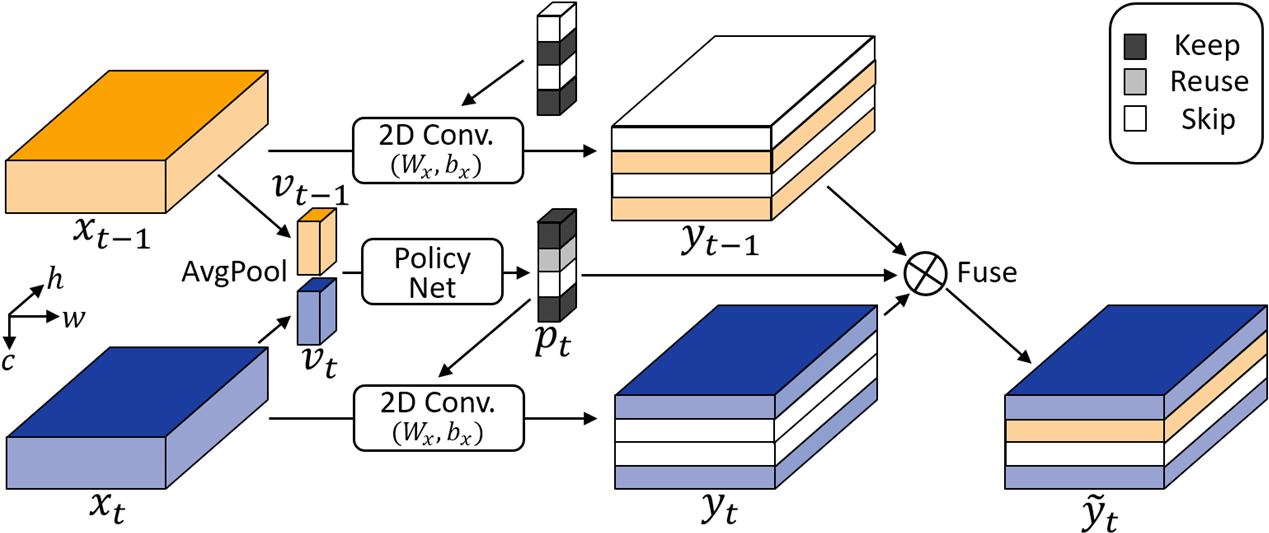
\includegraphics[width=8cm]{assets/shit.png}
	\caption{The agent of AdaFuse selects which channels to use dynamically.}
	\label{fig:imgs}
\end{figure}

\section{Method}
\subsection{2D-CNN for Action Recognition}
For action recognition, many methods first extract feature maps from each frame using 2D-CNN ($\mathcal{F}$) and colligate the feature maps using a consensus operation ($\mathcal{G}$) used for final prediction. So, the final prediction can be written as follows:
\begin{align*}
	P(X_1, ..., X_T) = \mathcal{G}(\mathcal{F}(X_1), ...,\mathcal{F}(X_T))
\end{align*}
where $T$ is the number of sampled frames, and $\{X_1, ..., X_T\}$ are the sampled frames. The consensus operation can be an average operation or LSTM. AdaFuse is inserted in between layers of $\mathcal{F}$.

\subsection{Adaptive Temporal Fusion}
Assume that $x_t \in \mathbb{R}^{c \times h \times w}$ is a feature map, and $y_t=\text{conv}(x_t) \in \mathbb{R}^{c' \times h' \times w'}$ is a feature map of the next layer. We define $v_t = GAP(x_t) \in \mathbb{R}^{c}$ as a global average pooled feature. AdaFuse adopts an agent $g$ that takes $v_t$ and $v_{t-1}$ and outputs $p_t \in \{0, 1, 2\}^{c}$ where $p_t$ is used to fuse $y_t$ and $y_{t-1}$:
\begin{align*}
	\hat{y}^i_t = \mathbf{1}[p^i_t = 0] \cdot y^i_t + \mathbf{1}[p^i_t = 1] \cdot y^i_{t-1}
\end{align*}
where $\mathbf{1}$ is the indicator function. We can interpret the equation as follows: if $p^i_t$ is 0, then we use the $i$-th channel of $y_t$; else if $p^i_t$ is 1, we use the $i$-th channel of $y_{t-1}$; finally, if $p^i_t$ is 2, we mask the $i$-th channel as zeros (Figure~\ref{fig:imgs}). 

\subsection{Loss functions}
The loss function is the sum of the cross-entropy loss and the FLOPS of AdaFuse layers. The agent learns to minimize the FLOPS while maintaining the accuracy.

\section{Results}
The authors evaluate the effectiveness of the proposed method on various datasets such as Something-Something V1, Jester, and Mini-Kinetics. 
AdaFuse consistently improves performance while maintaining the FLOPS of the network, and in some experiments, the method shows better performance while reducing the FLOPS drastically. 

\section{Personal Note}
Even though integrating with Reinforce learning seems a little bit complicated, the method seems simple, neat, and efficient. 

% {\small
% \bibliographystyle{ieee}
% \bibliography{egbib}
% }


\end{document}
